\section{Introducción}
	\subsection{Motivación}
	En el vertiginoso avance de la tecnología, la aplicación de redes neuronales en el procesamiento de imágenes ha emergido como un catalizador revolucionario en diversas disciplinas. Entre las múltiples facetas que abarca esta amalgama de inteligencia artificial y visión computarizada, la detección y clasificación de señales de tránsito se destaca como un campo de estudio de gran relevancia e impacto práctico.
La seguridad vial es una preocupación global de suma importancia, y el tráfico vehicular se presenta como un escenario dinámico y complejo donde la correcta interpretación de señales juega un papel crucial. La detección automatizada y la clasificación precisa de señales de tránsito no solo pueden potenciar la eficiencia de los sistemas de transporte, sino que también desempeñan un papel esencial en la prevención de accidentes y la mejora de la movilidad urbana.
	\begin{figure}[ht]
		\centering
		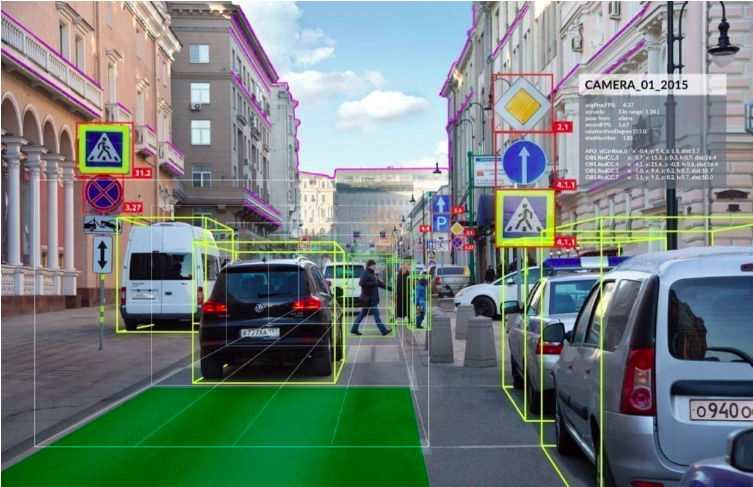
\includegraphics[height=7cm]{3}
		\caption{Reconocimiento de Objetos.}
	\end{figure}
	
El crecimiento exponencial de datos visuales en entornos urbanos y la necesidad de respuestas rápidas ante señales cambiantes hacen imperativa la adopción de enfoques avanzados. Acá es donde las redes neuronales toman importancia, porque su capacidad para aprender patrones complejos a partir de grandes conjuntos de datos permite el desarrollo de modelos capaces de discernir con precisión las señales de tráfico en imágenes, incluso en condiciones adversas.
En este contexto, la motivación subyacente es impulsar la aplicación de redes neuronales en el ámbito específico de la detección y clasificación de señales de tránsito.

\subsection {Objetivos}
	Los objetivos del proyecto son los siguientes:
	\begin{enumerate}
		\item \textbf{Pre-procesamiento de los datos:} Se llevará a cabo un pre-proceso en los datasets que tendrán relevancia en el entrenamiento de los distintos modelos.
		\item \textbf{Implementación de Arquitecturas Neuronales:}
		\begin{enumerate}
			\item \textbf{Desarrollo del modelo VGG-16:} Desarrollar la arquitectura de la red neuronal VGG-16 para la obtención de mapas de características, quitando capas para obtener resultados que necesitaremos para la siguiente etapa.
			\item \textbf{Desarrollo del modelo ROI-Pooling:}
				\begin{itemize}
					 \item Diseñar la arquitectura de la red neuronal ROI Pooling para identificar la presencia de señales de tránsito en los mapas de características obtenidos por VGG-16.
					 \item Entrenar la red ROI Pooling con diversos conjuntos de mapas de características generados a partir de imágenes de tráfico.
				\end{itemize}
			\item \textbf{Implementación del modelo de clasificación:}
				\begin{itemize}
					\item Investigación y evaluación de diferentes arquitecturas de redes neuronales. Se seleccionará la arquitectura más adecuada para el clasificador de señales de tránsito, teniendo en cuenta la precisión, la eficacia computacional y el tamaño del modelo.
					\item Entrenar la red de clasificación utilizando un conjunto de datos exclusivo que incluye imágenes de señales de tránsito etiquetadas.
				\end{itemize}
		\end{enumerate}
		\item \textbf{Integración de las redes neuronales:} Integrar las arquitecturas VGG-16, ROI Pooling y la red de clasificación para formar un modelo coherente y funcional de clasificación de señales de tránsito.
		\item \textbf{Evaluación del rendimiento del modelo:} Evaluar la precisión y eficacia del modelo completo mediante métricas relevantes de clasificación.
		\item \textbf{Comunicación:} Analizar críticamente los resultados, identificar posibles mejoras y proporcionar recomendaciones para futuras investigaciones.
	\end{enumerate}

\clearpage

%----------------------------------------------------------------------------------------
%	MARCO TEÓRICO
%----------------------------------------------------------------------------------------
\section{Marco Teórico}
	\subsection{Detección de Objetos}
	La detección de objetos constituye una rama esencial en el campo del procesamiento de imágenes y la visión por computadora. Su objetivo principal es discernir y localizar la presencia de uno o más objetos dentro de una imagen completa, asignándoles una identidad específica.
Las técnicas de detección de objetos se han desarrollado de manera significativa en respuesta a la creciente necesidad de sistemas capaces de comprender y responder a entornos visuales complejos. Uno de los enfoques más destacados y exitosos en este ámbito es el uso de redes neuronales convolucionales (CNN), que han demostrado una eficacia excepcional en la extracción de características relevantes de las imágenes.
La arquitectura típica para la detección de objetos a menudo involucra dos etapas cruciales: la generación de propuestas y la clasificación de esas propuestas. En la primera etapa, se utilizan técnicas como Region Proposal Networks (RPN) para proponer regiones de interés que podrían contener objetos. Posteriormente, estas regiones son clasificadas y refinadas utilizando capas de clasificación y regresión.

	\begin{figure}[ht]
	    \centering
		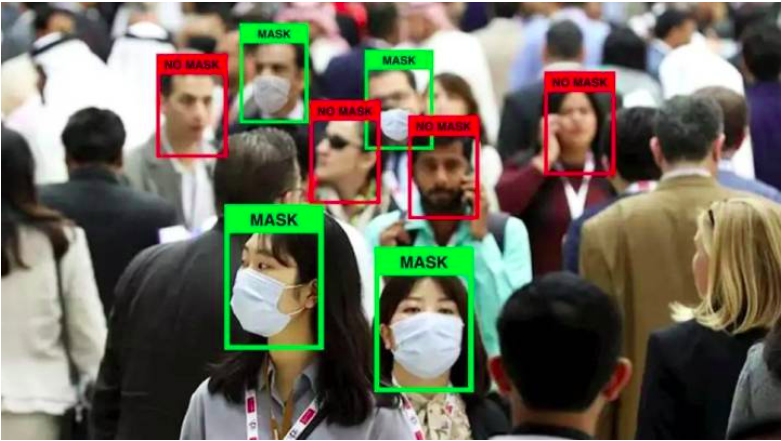
\includegraphics[scale=.4]{4}
		\caption{Reconocimiento facial}
	\end{figure}		
	
	Un enfoque más reciente y potente en la detección de objetos es la utilización de modelos de detección de objetos de una sola etapa, como YOLO (You Only Look Once) y SSD (Single Shot Multibox Detector). Estos modelos permiten la detección de objetos en tiempo real al abordar la tarea de manera conjunta, prediciendo las clases y las ubicaciones de los objetos de una sola vez.
Además, existen distintos tipos de detecciones y clasificaciones:
	\begin{itemize}
		\item Clasificación de la imagen.
		\item Clasificación con Localización.
		\item Detección.
	\end{itemize}

	\subsection{Clasificación de la imágen}
	En líneas generales, la clasificación de imágenes implica el uso de CNN seguidas de capas totalmente conectadas. Estas redes convolucionales son particularmente eficientes en la extracción de características relevantes, como bordes, texturas y patrones, mientras que las capas totalmente conectadas permiten la interpretación global de estas características para realizar la clasificación final.
Por ejemplo, en el contexto específico de la detección de vehículos, el objetivo de la clasificación se centraría en determinar la probabilidad de que la imagen contenga un automóvil. Esta probabilidad se obtiene al alimentar la imagen a través de la red neuronal, que ha sido previamente entrenada para reconocer patrones asociados con la presencia de vehículos.
	\begin{figure}[ht]
	    \centering
		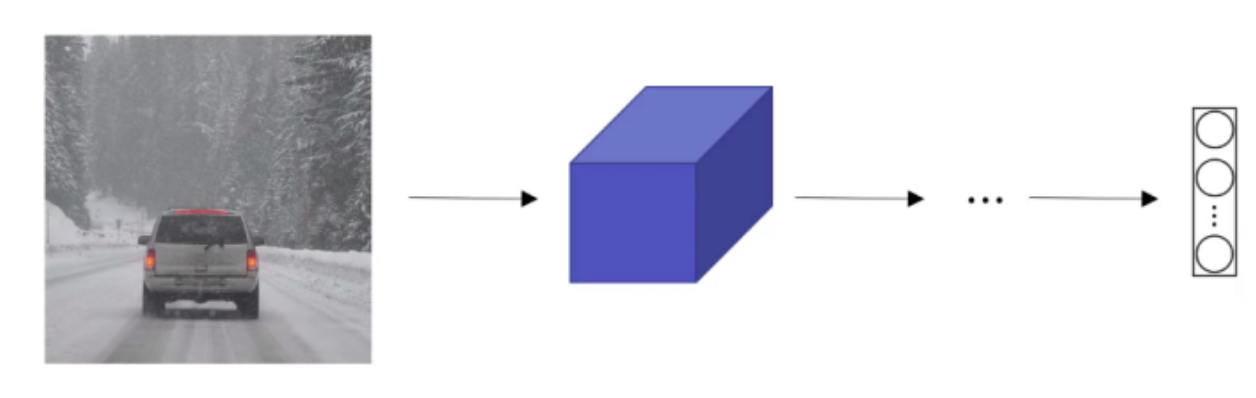
\includegraphics[scale=.30]{5}
		\caption{Representación del proceso de clasificación}
	\end{figure}

	\subsection{Clasificación con Localización}
	Para refinar aún más esta tarea, se pueden agregar neuronas de salida adicionales que proporcionen información sobre la localización del vehículo. Este enfoque, a menudo utilizado en sistemas de detección y clasificación de objetos, utiliza una bounding box (caja delimitadora) para representar la región en la que se encuentra el objeto de interés. En el caso de la detección de vehículos, esta \texttt{bounding box} se define mediante cuatro valores: \textbf{bx} (coordenada x del centro), \textbf{by} (coordenada y del centro), \textbf{bh} (altura) y \textbf{bw} (ancho)
	
	\begin{figure}[ht]
	    \centering
		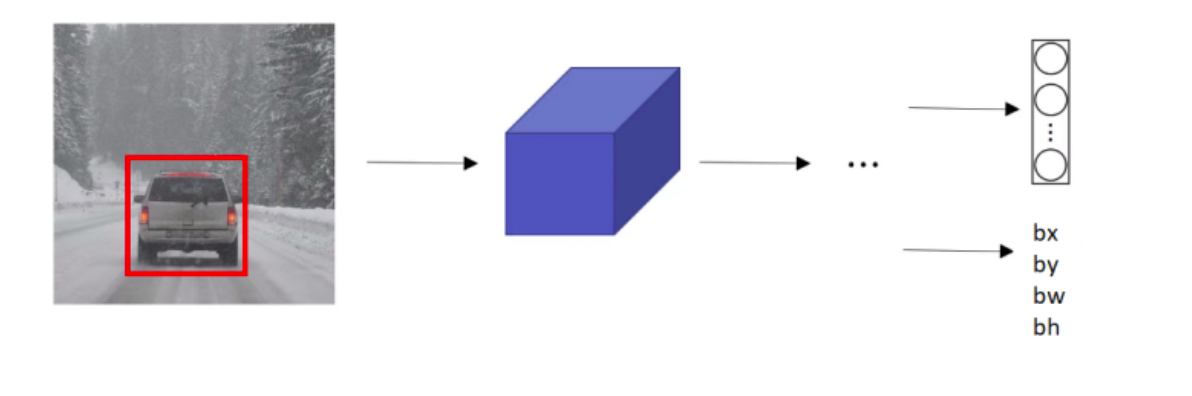
\includegraphics[scale=.35]{6}
		\caption{Representación del proceso de clasificación con localización}
	\end{figure}
	
	La inclusión de esta información espacial permite no solo identificar la presencia de un vehículo en la imagen, sino también delimitar su ubicación precisa. Este enfoque, combinado con técnicas avanzadas de clasificación, potencia la capacidad del sistema para comprender la escena visual en su totalidad y, en el caso específico de la detección de vehículos, proporcionar información detallada sobre su posición en la imagen.
	
	Por ejemplo, la salida de la red de clasificación con localización, considerando tres clases de objetos diferentes, sería la siguiente:
	
	\begin{center}
		\large{$y = [p_c$ $b_x$ $b_y$ $b_w$ $c_1$ $c_2$ $c_3]^T$}
	\end{center}
	
	Si ahora planteamos la función de pérdida de la salida (con MSE) tenemos:
	\vspace{0.3cm}
	\begin{itemize}[left=2cm]
	
	\item Si $p_c=1$
	\end{itemize}
	
	\begin{center}
		\large{$L(y,\hat{y}) = (\hat{y_1}-y_1)^2 + (\hat{y_2}-y_2)^2 +$ \dots $+ (\hat{y_8}-y_8)^2$}
	\end{center}	
		
	\begin{itemize}[left=2cm]
	\item Si $p_c=0$
	\end{itemize}
	
	\begin{center}
		\large{$L(y,\hat{y}) = (\hat{y_1}-y_1)^2$}
	\end{center}
	\pagebreak
	Por lo general se utiliza la función de pérdida log likelihood para las clases, mse para las coordenadas de la región limitante y logistic regression para $p_c$.

	\subsection{Etapa de la detección de objetos}
	En el campo de la detección de objetos, las arquitecturas aplicadas a menudo se estructuran en dos etapas distintas, cada una desempeñando un papel crucial en el proceso global de reconocimiento y localización de objetos en imágenes. Estas etapas son la detección de la región y la detección y clasificación del objeto.

	\begin{enumerate}
		\item Detección de la Región:
En la primera etapa, la detección de la región se centra en identificar áreas candidatas que podrían contener objetos de interés. Diversas técnicas han sido desarrolladas para esta tarea, entre las cuales se destacan la ventana deslizante y la búsqueda selectiva, entre otras similares. La ventana deslizante implica el escaneo sistemático de la imagen mediante una ventana móvil, evaluando cada región para determinar la probabilidad de contener un objeto. Por otro lado, la búsqueda selectiva utiliza propuestas generadas previamente para enfocarse en áreas más prometedoras de la imagen, reduciendo así la carga computacional.

	\item Detección y Clasificación del Objeto:
Una vez identificadas las regiones de interés, la siguiente etapa involucra la detección y clasificación del objeto dentro de estas regiones. Aquí, se pueden utilizar clasificadores clásicos o redes neuronales convolucionales entrenadas específicamente para reconocer patrones visuales asociados con categorías de objetos. Este paso es esencial para asignar una etiqueta a cada objeto detectado, proporcionando información sobre su naturaleza y características
	
	\end{enumerate}	

	\begin{figure}[ht]
	    \centering
		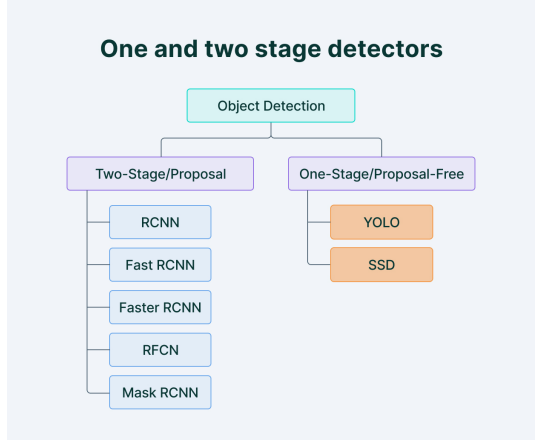
\includegraphics[scale=.47]{11}
		\caption{Esquema de detectores por etapas}
	\end{figure}
	
	\subsubsection{Arquitecturas Integradas}
	Aunque las dos etapas mencionadas anteriormente son comunes, han surgido arquitecturas más avanzadas que realizan ambas tareas simultáneamente. Estas arquitecturas integran la detección de la región y la clasificación del objeto en una única red neuronal, permitiendo una inferencia más eficiente y rápida.
En el panorama de la detección de objetos, la elección entre arquitecturas de una o dos etapas depende de los requisitos específicos de la aplicación y las limitaciones computacionales.

	\begin{figure}[ht]
	    \centering
		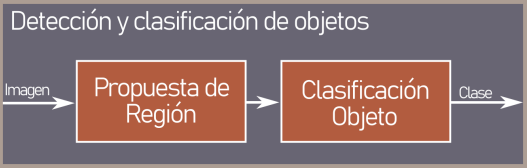
\includegraphics[scale=.5]{12}
		\caption{Arquitectura con dos etapas}
	\end{figure}
	
	\subsection{Ventana deslizante}
	La técnica de ventana deslizante, que implica el desplazamiento de rectángulos a través de una imagen en busca de objetos, se convierte en una estrategia aún más potente cuando se incorporan optimizaciones clave. Este enfoque exhaustivo se beneficia de la flexibilidad para cambiar el tamaño de la imagen o de la propia ventana deslizante, permitiendo la obtención de cajas de delimitaciones más precisas.
	
	\begin{figure}[ht]
  		\centering
  		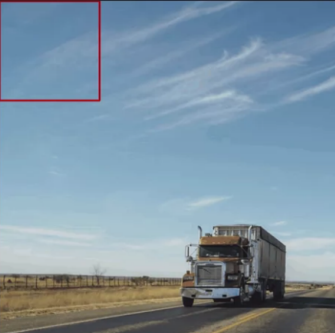
\includegraphics[width=0.25\textwidth]{13}
  		\hspace{0.5cm}
  		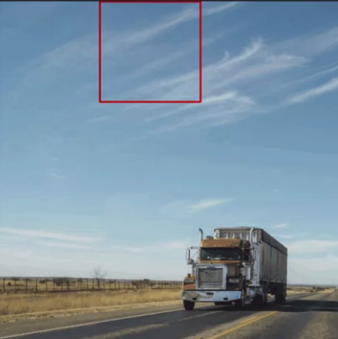
\includegraphics[width=0.25\textwidth]{14}
  		\caption{Representación de la técnica}
	\end{figure}

	Cuando se trabaja con imágenes de tamaños variados, ajustar la escala de la ventana deslizante es esencial para garantizar la detección efectiva de objetos en diferentes contextos. Posteriormente, basándose en las ventanas donde se detecta el objeto en imágenes más pequeñas, se puede escalar nuevamente y unir las detecciones. Este proceso contribuye significativamente a obtener resultados más precisos y detallados, especialmente en escenarios donde la escala de los objetos varía considerablemente.

	\begin{figure}[ht]
	    \centering
		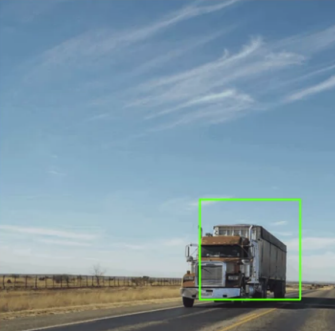
\includegraphics[scale=.33]{15}
		\caption{Representación de la técnica}
	\end{figure}

	La versatilidad de la ventana deslizante también puede conducir a situaciones en las que varias cajas de delimitaciones detectan el mismo objeto. El desafío radica en seleccionar la mejor candidata entre estas detecciones redundantes. Para abordar este problema, se emplea la técnica de \textbf{Non-Maximum Suppression} (supresión de no máximos) entre las candidatas. Esta estrategia se centra en retener únicamente la detección más confiable, descartando las demás para evitar duplicaciones innecesarias.
	
	\begin{figure}[ht]
	    \centering
		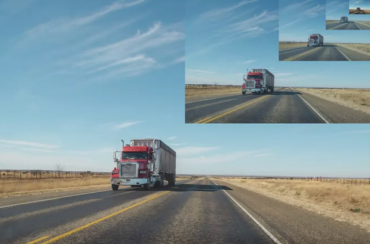
\includegraphics[scale=.45]{16}
		\caption{Representación de la técnica NMS}
	\end{figure}
	
	La evaluación de la calidad de las detecciones se realiza mediante la métrica Intersection Over Union (Intersección sobre Unión, IoU). Esta métrica calcula la proporción entre la intersección y la unión de dos regiones delimitadas por cajas. Al establecer un umbral específico de IoU, se puede determinar la superposición aceptable entre dos cajas para considerarlas como duplicadas o no. Esto asegura que la mejor candidata seleccionada sea la que mejor se ajusta a la verdadera posición y forma del objeto.

	\begin{figure}[ht]
	    \centering
		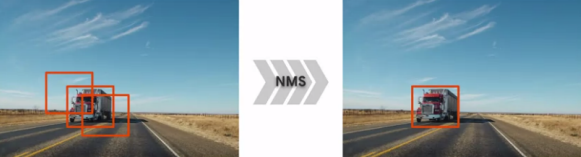
\includegraphics[scale=.55]{18}
		\caption{Representación de la técnica NMS}
	\end{figure}
	
	\subsubsection{Otros datos}
	La técnica de ventana deslizante, a pesar de ser efectiva en la detección de objetos, enfrenta desafíos computacionales significativos, especialmente en términos de eficiencia. Su alto costo computacional se debe a que cada recorte generado por el desplazamiento de la ventana debe procesarse individualmente por la red convolucional, siendo más intensivo en recursos con imágenes de alta resolución o detecciones más precisas.

	La situación empeora al buscar un desplazamiento más preciso, ya que explorar un espacio de búsqueda más fino implica procesar más regiones, aumentando exponencialmente la carga computacional. La ventana deslizante no es óptima para Redes Neuronales Convolucionales (CNN), ya que la complejidad de las CNN hace que el procesamiento independiente de cada recorte sea ineficiente y costoso.

	Para superar estas limitaciones, se propone la ventana deslizante convolucional, que optimiza el proceso al introducir la convolución directamente en la ventana. Esto permite a la red compartir cálculos entre regiones superpuestas, reduciendo redundancias y mejorando la eficiencia global del modelo.

	\subsection{Intersección sobre la Union (IoU)}
	La métrica de Intersección sobre la Unión (IoU) es un elemento crucial en la evaluación de la precisión y calidad de las predicciones en la detección de objetos. Esta métrica proporciona una medida del grado de superposición entre dos regiones delimitantes, ofreciendo una indicación clara de la similitud y, por ende, de la efectividad del modelo predictivo.

    
	El cálculo de IoU está dado por la siguiente expresión:
	
	\begin{equation*}
    	IoU = \frac{\text{área de la intersección}}{\text{área de la unión}}
	\end{equation*}
	
	Donde el numerador representa el área compartida entre las dos regiones delimitantes, y el denominador representa el área total cubierta por ambas. Este cálculo proporciona un valor normalizado que varía entre 0 y 1, donde 0 indica ninguna superposición y 1 indica una coincidencia perfecta entre las regiones.
	
	\vspace{0.3cm}
	
	\textbf{La interpretación del resultado de IoU es directa:} 
	\begin{itemize}
	\item A medida que el valor de IoU se acerca a 1, se indica una mayor similitud y precisión en la predicción
	\item Un IoU de 0.5 se considera un umbral comúnmente aceptado para determinar si una predicción es correcta
	\item Si el IoU es mayor a 0.5, se considera que la predicción es precisa, lo que implica que la región predicha se superpone significativamente con la región real del objeto.
	
	\end{itemize}		

	Esta métrica es especialmente valiosa en situaciones donde es esencial evaluar no solo la detección de un objeto, sino también la precisión de su ubicación y forma predicha. Al establecer un umbral significativo, se puede establecer un estándar para la aceptabilidad de las predicciones, contribuyendo así a la toma de decisiones en la optimización de modelos de detección de objetos.

	\begin{figure}[ht]
	    \centering
		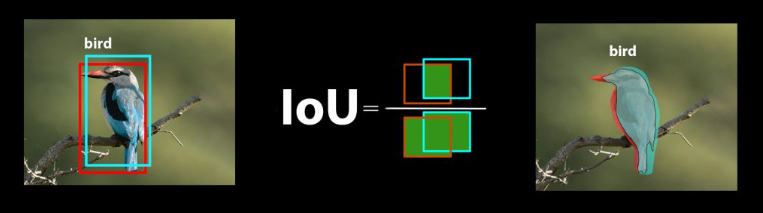
\includegraphics[scale=.55]{35}
		\caption{Representación de la métrica IoU}
	\end{figure}

	\subsection{Non-Max Supression}

	\begin{wrapfigure}[16]{R}{.40\textwidth} 
		\centering
		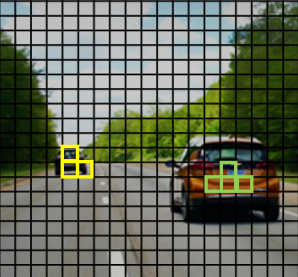
\includegraphics[scale=.50]{19}
		\caption{Referencia a la técnica NMS}
	\end{wrapfigure}
	
	La técnica de Non-Maximum Suppression (NMS) es una estrategia esencial en el postprocesamiento de detecciones, particularmente cuando se enfrenta a la presencia de múltiples celdas o ventanas que comprenden un solo objeto. El objetivo principal de NMS es seleccionar la ventana que mejor encuadre al objeto en cuestión, eliminando redundancias y asegurando una salida precisa.
    El proceso de Non-Maximum Suppression inicia evaluando las probabilidades asociadas con cada detección (pc) y seleccionando la ventana con la probabilidad más alta. Este paso inicial garantiza que la predicción más confiable se mantenga, sirviendo como referencia para la supresión de detecciones redundantes.
	
	Se calcula el valor de solapamiento (IoU) entre estos rectángulos y el rectángulo de mayor probabilidad. 


	\begin{wrapfigure}[15]{L}{.36\textwidth} 
		\centering
		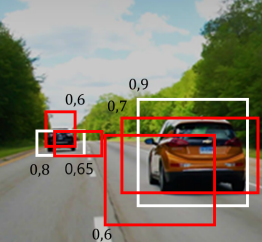
\includegraphics[scale=.52]{20}
		\caption{Representación NMS-IOU}
	\end{wrapfigure}

    Aquellos rectángulos que tienen un valor de IoU significativo con el rectángulo de referencia son suprimidos, ya que representan detecciones superpuestas o redundantes. 
    
    Este proceso, además de supresión, garantiza que solo se retenga la detección más confiable y precisa, eliminando aquellas que no aportan información adicional significativa. La técnica de Non-Maximum Suppression, por lo tanto, contribuye a la generación de resultados más limpios y coherentes en el contexto de la detección de objetos.

    
    Es importante destacar que, en escenarios donde hay varios objetos a detectar, NMS puede ejecutarse de manera independiente para cada salida, permitiendo así un manejo eficiente de múltiples detecciones en una única imagen, y así asegurando que la selección de ventanas se realice de manera óptima para cada objeto individual.	
 	
	A pesar de la optimización que proporciona la implementación de la técnica de ventana deslizante en conjunto con redes neuronales convolucionales (CNN), surge una limitación.

	Esta limitación se manifiesta en situaciones donde ninguna ventana deslizante coincide de manera precisa con la posición real del objeto, como un vehículo. Además, la forma y tamaño predeterminados de la ventana deslizante pueden no ser los más apropiados para delimitar con precisión la región de interés.
	
	La falta de precisión en los límites del cuadro delimitador puede comprometer la exactitud global del sistema de detección de objetos. Esto se convierte en un desafío importante, ya que la correcta delimitación de la región ocupada por el objeto es esencial para comprender su ubicación y forma con precisión.
	Para abordar esta limitación, se exploran enfoques avanzados que buscan mejorar la predicción de los cuadros delimitadores, permitiendo una detección más precisa y detallada de los objetos en la imagen. Estos enfoques a menudo involucran técnicas de regresión que buscan ajustar dinámicamente los límites del cuadro en función de las características específicas del objeto detectado.

	\subsection{R-CNN}
	
	\begin{wrapfigure}[18]{R}{.43\textwidth} 
		\centering
		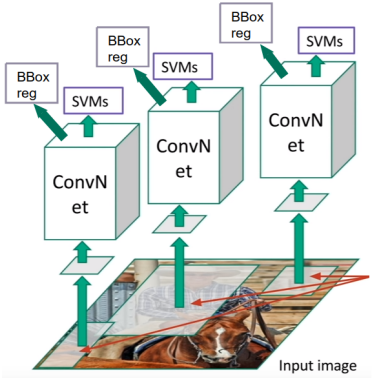
\includegraphics[scale=.40]{26}
		\caption{Representación de R-CNN}
	\end{wrapfigure}

	El enfoque R-CNN es una metodología que incorpora redes neuronales convolucionales (CNN) basadas en regiones para implementar la búsqueda selectiva de objetos en una imagen.
El proceso R-CNN inicia con la fase de búsqueda selectiva, donde se exploran alrededor de 2000 posibles regiones de interés en la imagen. Esta etapa utiliza la técnica de búsqueda selectiva para identificar áreas prometedoras que podrían contener objetos de interés. Esta primera fase de selección de regiones es esencial para reducir la complejidad computacional y centrar el análisis en áreas relevantes.

	Posteriormente, cada región seleccionada se somete a un proceso de extracción de características utilizando una red neuronal pre-entrenada. Esta red, habitualmente diseñada para tareas de clasificación de imágenes a gran escala, se adapta para capturar las características específicas de las regiones de interés. Esta adaptación permite que la red aprenda representaciones significativas de los objetos contenidos en las regiones, contribuyendo a una detección más precisa.

	\subsection{Fast R-CNN}
	Para superar las limitaciones de velocidad inherentes a la arquitectura R-CNN, surge Fast R-CNN. R-CNN, aunque efectiva, enfrenta desafíos computacionales significativos debido a su técnica de búsqueda selectiva en toda la imagen y al procesamiento lento de 2000 áreas de interés a través de las CNN.
Fast R-CNN aborda estas limitaciones implementando una estrategia más eficiente. En lugar de enviar cada región de interés por separado a la red neuronal, Fast R-CNN integra una CNN que opera en toda la imagen. Esta CNN de toda la imagen extrae características generales y crea feature maps que luego se utilizan para cada región de interés.
Esta arquitectura optimizada ahorra tiempo y recursos computacionales al evitar el procesamiento repetitivo de la imagen completa para cada región. Al utilizar feature maps compartidos, Fast R-CNN logra una mayor eficiencia en la extracción de características, permitiendo una detección más rápida y precisa de objetos en la imagen.

	\begin{figure}[ht]
	    \centering
		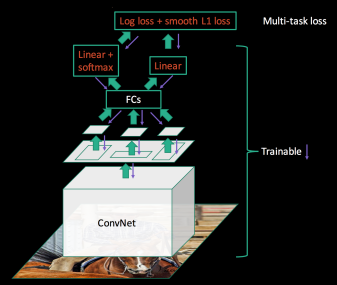
\includegraphics[scale=.60]{27}
		\caption{Representación de Fast R-CNN}
	\end{figure}
	
	\subsection{Faster R-CNN}
	
	\begin{wrapfigure}[16]{R}{.43\textwidth} 
		\centering
		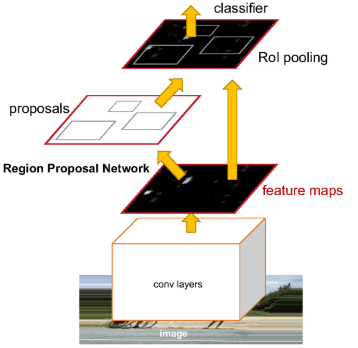
\includegraphics[scale=.40]{28}
		\caption{Representación de Faster R-CNN}
	\end{wrapfigure}
	
	Faster R-CNN integra de manera eficiente el algoritmo de proposición de regiones de interés directamente en la red neuronal convolucional (CNN).
	
	La principal innovación de Faster R-CNN radica en su capacidad para unificar el enfoque eficiente de extracción de características de Fast R-CNN con un algoritmo de proposición de regiones, creando así una arquitectura integral y ágil. Esta integración permite que la red proponga automáticamente las regiones de interés, eliminando la necesidad de procesos separados y mejorando drásticamente la eficiencia del modelo.


	Comparado con su predecesor, R-CNN, Faster R-CNN se destaca por su velocidad. Es 250 veces más rápido que R-CNN, y supera significativamente a Fast R-CNN siendo 25 veces más rápido. Estas mejoras en velocidad no solo aceleran el proceso de detección, sino que también abren posibilidades para la implementación de sistemas en tiempo real y aplicaciones de visión por computadora más exigentes.
	
	\subsection{YOLO(You Only Look Once)}
	\subsubsection{Algoritmo}
	YOLO lleva a cabo la detección de objetos realizando la clasificación y localización en un solo paso. Su enfoque consiste en dividir la imagen en una cuadrícula SxS y prever, para cada elemento de la cuadrícula, N áreas de detección con un porcentaje de confianza asociado.
	
	En total, YOLO predice SxSxN áreas, pero aplica un filtro, descartando aquellas con baja confidencia. Esta estrategia de filtrado contribuye a la generación de predicciones más precisas y confiables, centrándose en áreas con una alta probabilidad de contener objetos de interés.
	
	\begin{figure}[ht]
			\centering
			\begin{subfigure}[t]{.47\textwidth}
				\centering
				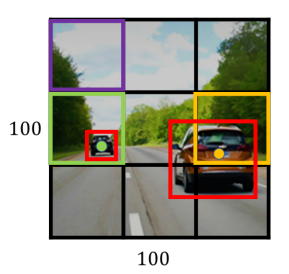
\includegraphics[scale=.50]{30}
			\end{subfigure}
			\begin{subfigure}[t]{.47\textwidth}
				\centering
				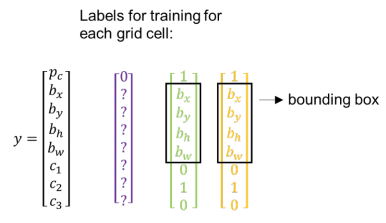
\includegraphics[scale=.50]{31}
			\end{subfigure}
			\caption{Representación de uso de la técnica}
			\end{figure}		
		
	Esta técnica única combina la ventana deslizante con la clasificación y localización, superando las limitaciones de enfoques anteriores.
	
	En YOLO, el objeto se asigna a la celda que contiene el punto central del área de detección, proporcionando una localización más precisa y simplificando el proceso de detección.
	
	Ahora bien, en la arquitectura YOLO, se implementa una estrategia que utiliza dos o más áreas de detección por celda. Aunque en una celda solo se puede detectar un objeto, la introducción de múltiples cajas permite que cada una se ``especialice'' en aprender diferentes relaciones y tamaños de objetos. Este enfoque polivalente mejora significativamente la capacidad de YOLO para adaptarse a la diversidad de objetos presentes en una imagen. Cada área de detección contribuye con su propia percepción y comprensión, permitiendo que el modelo aborde eficazmente objetos de distintas escalas y formas.
	
	\begin{figure}[ht]
		\centering
		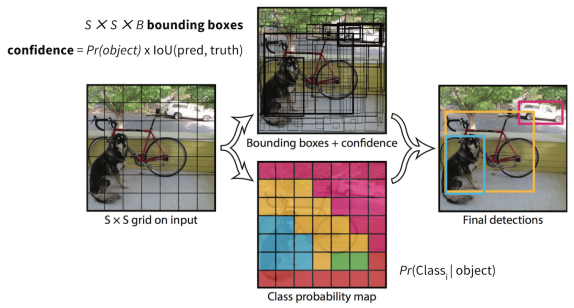
\includegraphics[scale=.6]{32}
		\caption{Ejemplo de uso}
	\end{figure}
	
	La dimensión de salida de YOLO se define como $S*S*(5B+K)$, donde S representa el tamaño de la cuadrícula, B denota el número de cajas de detección por celda, y K es la cantidad de clases de objetos a prever. Este diseño compacto y expresivo es fundamental para la eficiencia y versatilidad del algoritmo.
	

	\subsubsection{Arquitectura}
	La arquitectura de YOLO está organizada en tres etapas fundamentales que abarcan desde la extracción de características hasta la generación de predicciones y el posterior post procesamiento:
		
	\begin{enumerate}
    	\item \textbf{Backbone:} En la primera etapa, YOLO utiliza una red neuronal preentrenada como su espina dorsal o \textit{backbone}. Ejemplos comunes incluyen DarkNet. Esta fase se encarga de extraer características fundamentales de la imagen, aprovechando el conocimiento previo obtenido durante el entrenamiento de la red.

    	\item \textbf{Neck:} La etapa del cuello se caracteriza por capas completamente conectadas que reciben las características extraídas por la espina dorsal. Estas capas se encargan de fusionar y combinar las representaciones de características para capturar información más compleja y contextual. Esta fase actúa como un puente entre la espina dorsal y la capa de salida.

    	\item \textbf{Head:} La última etapa, la cabeza, consiste en la capa de salida que produce las predicciones finales. Aquí se generan las coordenadas de las cajas delimitadoras, las puntuaciones de confianza asociadas a cada detección y las probabilidades de clasificación para las clases de objetos. Además, se aplica el postprocesamiento, que incluye Non-Maximum Suppression (NMS) y el cálculo del Índice de Superposición de Unión (IoU). Estos pasos finales mejoran la precisión y la consistencia de las detecciones, asegurando que se retenga la predicción más confiable y precisa para cada objeto en la imagen.
	\end{enumerate}

	\begin{figure}[ht]
		\centering
		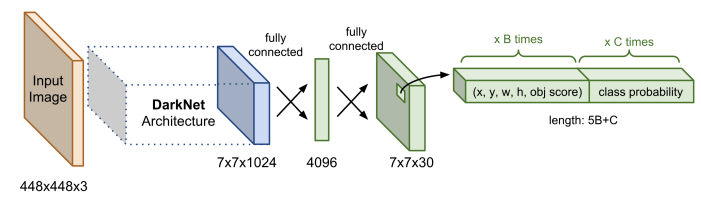
\includegraphics[scale=.6]{33}
		\caption{Ejemplo de arquitectura}
	\end{figure}
	
	\subsubsection{Entrenamiento - Función Pérdida}
	La función de pérdida en la arquitectura YOLO se segmenta en dos componentes fundamentales:
	
	\begin{enumerate}
		\item Pérdida por la predicción del área delimitante $(x, y, h, w)$: $L_loc$
		\item Pérdida por la clasificación del objeto: $L_cls$
	\end{enumerate}
	
	Ambas pérdidas se calculan utilizando el error cuadrático medio (MSE), y cada una de ellas incorpora dos parámetros de escala cruciales: $\lambda_coor$ y $\lambda_noobj$. Estos parámetros influyen en la importancia relativa de cada término de pérdida, permitiendo un ajuste preciso del modelo en función de las metas específicas del entrenamiento.
	\\[0.5cm]
	\textbf{Pérdida en la localización:}
	\vspace{0.5cm}
	\begin{equation*}
		L_{loc} = \lambda_{coord} \sum_{i=0}^{S^2} \sum_{j=0}^{B} 1_{ij}^{obj} [(x_i-\hat{x_i})^2+(y_i-\hat{y_i})^2+(\sqrt{w_i}-\sqrt{\hat{w_i}})^2+(\sqrt{h_i}-\sqrt{\hat{h_i}})^2]
	\end{equation*}
	\vspace{0.1cm}
	\begin{itemize}
		\item \textbf{S}: Cantidad de celdas.
		\item \textbf{B}: Cantidad de áreas de delimitación por celda.
		\item \( \mathbf{1_{ij}^{obj}} \):Indica que el área de delimitación j de la celda i es responsable de la predicción.
	\end{itemize}
	
	\clearpage
	
	\textbf{Pérdida en la clasificación:}
	\vspace{0.5cm}
	\begin{equation*}
		L_{cls} = \lambda_{coord} \sum_{i=0}^{S^2} \sum_{j=0}^{B} (1_{ij}^{obj}+ \lambda_{noobj}(1-1_{ij}^{obj}))(C_{ij}-\hat{C_{ij}})^2+\sum_{i=0}^{S^2} \sum_{c\in{C}} 1_{ij}^{obj}(p_i(c)-\hat{p_i}(c))^2 
	\end{equation*}
	
	\begin{equation*}
		L = L_{loc} + L_{cls}	
	\end{equation*}
	\vspace{0.1cm}
	
	\begin{itemize}
    \item \( \mathbf{1_{i}^{obj}} \): Indica que existe un objeto en la celda \(i\).
    \item \( \mathbf{1_{ij}^{obj}} \): Indica que el área de delimitación \(j\) de la celda \(i\) es responsable de la predicción.
    \item \( \mathbf{C_{ij} }\): Confianza de la celda $(Pr(obj) * IoU(pred, truth))$.
    \item \( \mathbf{\hat{C_{ij}}} \): Confianza de la celda predicha.
    \item \( \mathbf{p_i}(c) \) Probabilidad condicional de una celda \(i\) de contener un objeto de clase \(c\in{C}\).
    \item \( \mathbf{\hat{p_{i}}}(c)\) Probabilidad condicional de una celda \(i\) de contener un objeto de clase \(c\in{C}\) predicha por el modelo
\end{itemize}

	El coeficiente de escala de pérdida $\lambda_{noobj}$ desempeña un papel importante en la prevención de entrenamientos incorrectos, especialmente dado que la mayoría de las celdas en una cuadrícula no contendrán objetos. La determinación del predictor responsable se lleva a cabo mediante el cálculo de la Intersección sobre Unión (IoU). Además, durante el entrenamiento, se emplean cajas de anclaje (anchor boxes) para mejorar y ajustar el rendimiento del predictor.

	\begin{figure}[ht]
		\centering
		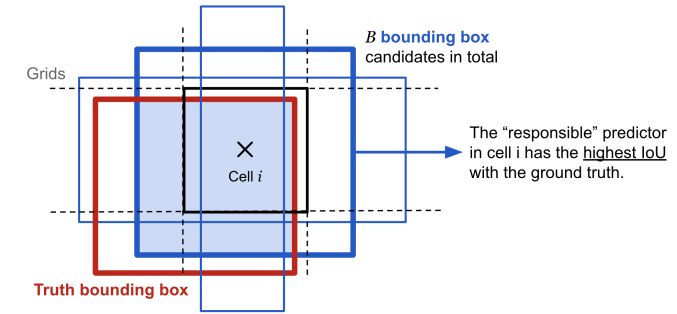
\includegraphics[scale=.6]{34}
		\caption{Representación de la técnica}
	\end{figure}
	
	\subsubsection{Ventajas}
	
	\begin{enumerate}
		\item \textbf{Eficiencia en Tiempo Real:} YOLO es conocido por su eficiencia en tiempo real, ya que realiza la detección de objetos en una sola pasada. Esto lo hace particularmente adecuado para aplicaciones en las que se requiere baja latencia, como en sistemas de vigilancia y conducción autónoma.
    
    	\item \textbf{Detección de Objetos Múltiples:} YOLO puede detectar múltiples objetos en una imagen, incluso aquellos de diferentes tamaños y clases. Su capacidad para manejar la diversidad en la detección es una de sus fortalezas clave.
    
   		\item \textbf{Sim­plicidad y Unificación:} YOLO unifica la clasificación y localización en un solo paso, simplificando el proceso de detección. Su diseño compacto facilita la implementación y el ajuste en diversas aplicaciones.
    
	\end{enumerate}
	
	\subsubsection{Desventajas}
	
	\begin{enumerate}
		\item \textbf{Precisión en Objetos Pequeños:} YOLO puede tener dificultades al detectar objetos pequeños debido a la resolución limitada de las áreas de detección y la pérdida de detalles en objetos diminutos.
    
    	\item \textbf{Manejo de Objetos Superpuestos:} En situaciones donde los objetos están superpuestos, YOLO puede enfrentar desafíos para distinguir y delimitar con precisión cada objeto individual.
    
   	 	\item \textbf{Problema de Clasificación Desbalanceada:} Si hay una gran variabilidad en la cantidad de instancias de diferentes clases en el conjunto de datos, puede haber desafíos asociados con el equilibrio en la clasificación.
    
    	\item \textbf{Entrenamiento Sensible a la Inicialización:} El rendimiento de YOLO puede depender en gran medida de una buena inicialización durante el entrenamiento, y un mal ajuste inicial podría afectar la calidad de las predicciones.	
	
	\end{enumerate}
	
	


	

<<<<<<< Updated upstream
	\subsection{R-CNN}
=======

     \begin{flushright}
        \textbf{Material Consultado \cite{filminasleo}.}
    \end{flushright}

	\subsection{Fast R-CNN}

	\begin{wrapfigure}[18]{R}{.43\textwidth} 
	    \centering
		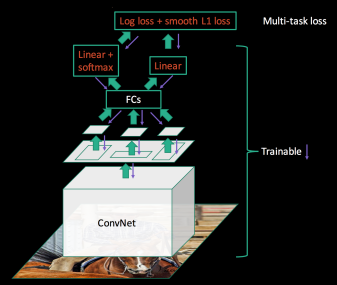
\includegraphics[scale=.5]{27}
		\caption{Representación de Fast R-CNN}
	\end{wrapfigure}
 
	Para superar las limitaciones de velocidad inherentes a la arquitectura R-CNN, surge Fast R-CNN. R-CNN, aunque efectiva, enfrenta desafíos computacionales significativos debido a su técnica de búsqueda selectiva en toda la imagen y al procesamiento lento de 2000 áreas de interés a través de las CNN.
 
    Fast R-CNN aborda estas limitaciones implementando una estrategia más eficiente. En lugar de enviar cada región de interés por separado a la red neuronal, Fast R-CNN integra una CNN que opera en toda la imagen. Esta CNN de toda la imagen extrae características generales y crea feature maps que luego se utilizan para cada región de interés.
    
    Esta arquitectura optimizada ahorra tiempo y recursos computacionales al evitar el procesamiento repetitivo de la imagen completa para cada región. Al utilizar feature maps compartidos, Fast R-CNN logra una mayor eficiencia en la extracción de características, permitiendo una detección más rápida y precisa de objetos en la imagen.
    \pagebreak

	\subsection{Faster R-CNN}
>>>>>>> Stashed changes
	
	\begin{wrapfigure}[17]{R}{.43\textwidth} 
		\centering
		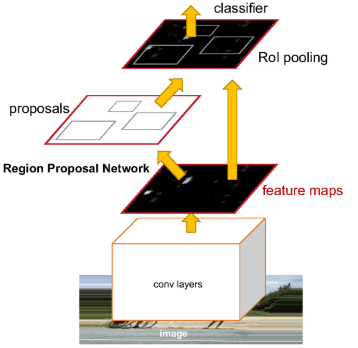
\includegraphics[scale=.44]{28}
		\caption{Representación de Faster R-CNN}
	\end{wrapfigure}
	
	Faster R-CNN integra de manera eficiente el algoritmo de proposición de regiones de interés directamente en la red neuronal convolucional (CNN).
	
	La principal innovación de Faster R-CNN radica en su capacidad para unificar el enfoque eficiente de extracción de características de Fast R-CNN con un algoritmo de proposición de regiones, creando así una arquitectura integral y ágil. Esta integración permite que la red proponga automáticamente las regiones de interés, eliminando la necesidad de procesos separados y mejorando drásticamente la eficiencia del modelo.


<<<<<<< Updated upstream
	\subsection{Fast R-CNN}
	Para superar las limitaciones de velocidad inherentes a la arquitectura R-CNN, surge Fast R-CNN. R-CNN, aunque efectiva, enfrenta desafíos computacionales significativos debido a su técnica de búsqueda selectiva en toda la imagen y al procesamiento lento de 2000 áreas de interés a través de las CNN.
Fast R-CNN aborda estas limitaciones implementando una estrategia más eficiente. En lugar de enviar cada región de interés por separado a la red neuronal, Fast R-CNN integra una CNN que opera en toda la imagen. Esta CNN de toda la imagen extrae características generales y crea feature maps que luego se utilizan para cada región de interés.
Esta arquitectura optimizada ahorra tiempo y recursos computacionales al evitar el procesamiento repetitivo de la imagen completa para cada región. Al utilizar feature maps compartidos, Fast R-CNN logra una mayor eficiencia en la extracción de características, permitiendo una detección más rápida y precisa de objetos en la imagen.

	\begin{figure}[ht]
	    \centering
		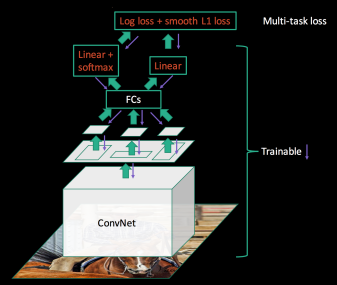
\includegraphics[scale=.60]{27}
		\caption{Representación de Fast R-CNN}
	\end{figure}
	
	\subsection{Faster R-CNN}
	
	\begin{wrapfigure}[16]{R}{.43\textwidth} 
		\centering
		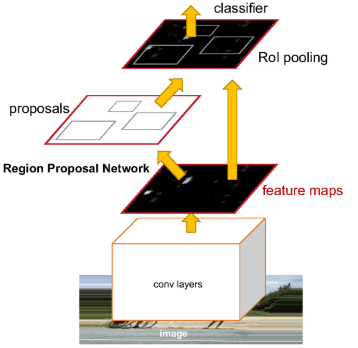
\includegraphics[scale=.40]{28}
		\caption{Representación de Faster R-CNN}
	\end{wrapfigure}
	
	Faster R-CNN integra de manera eficiente el algoritmo de proposición de regiones de interés directamente en la red neuronal convolucional (CNN).
	
	La principal innovación de Faster R-CNN radica en su capacidad para unificar el enfoque eficiente de extracción de características de Fast R-CNN con un algoritmo de proposición de regiones, creando así una arquitectura integral y ágil. Esta integración permite que la red proponga automáticamente las regiones de interés, eliminando la necesidad de procesos separados y mejorando drásticamente la eficiencia del modelo.


	Comparado con su predecesor, R-CNN, Faster R-CNN se destaca por su velocidad. Es 250 veces más rápido que R-CNN, y supera significativamente a Fast R-CNN siendo 25 veces más rápido. Estas mejoras en velocidad no solo aceleran el proceso de detección, sino que también abren posibilidades para la implementación de sistemas en tiempo real y aplicaciones de visión por computadora más exigentes.
	
	\subsection{YOLO(You Only Look Once)}
	\subsubsection{Algoritmo}
	YOLO lleva a cabo la detección de objetos realizando la clasificación y localización en un solo paso. Su enfoque consiste en dividir la imagen en una cuadrícula SxS y prever, para cada elemento de la cuadrícula, N áreas de detección con un porcentaje de confianza asociado.
	
	En total, YOLO predice SxSxN áreas, pero aplica un filtro, descartando aquellas con baja confidencia. Esta estrategia de filtrado contribuye a la generación de predicciones más precisas y confiables, centrándose en áreas con una alta probabilidad de contener objetos de interés.
	
	\begin{figure}[ht]
			\centering
			\begin{subfigure}[t]{.47\textwidth}
				\centering
				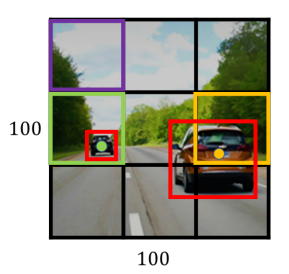
\includegraphics[scale=.50]{30}
			\end{subfigure}
			\begin{subfigure}[t]{.47\textwidth}
				\centering
				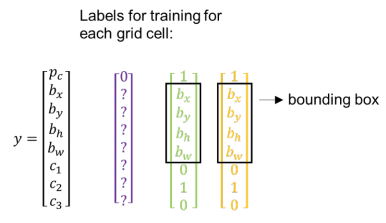
\includegraphics[scale=.50]{31}
			\end{subfigure}
			\caption{Representación de uso de la técnica}
			\end{figure}		
		
	Esta técnica única combina la ventana deslizante con la clasificación y localización, superando las limitaciones de enfoques anteriores.
	
	En YOLO, el objeto se asigna a la celda que contiene el punto central del área de detección, proporcionando una localización más precisa y simplificando el proceso de detección.
	
	Ahora bien, en la arquitectura YOLO, se implementa una estrategia que utiliza dos o más áreas de detección por celda. Aunque en una celda solo se puede detectar un objeto, la introducción de múltiples cajas permite que cada una se ``especialice'' en aprender diferentes relaciones y tamaños de objetos. Este enfoque polivalente mejora significativamente la capacidad de YOLO para adaptarse a la diversidad de objetos presentes en una imagen. Cada área de detección contribuye con su propia percepción y comprensión, permitiendo que el modelo aborde eficazmente objetos de distintas escalas y formas.
	
	\begin{figure}[ht]
		\centering
		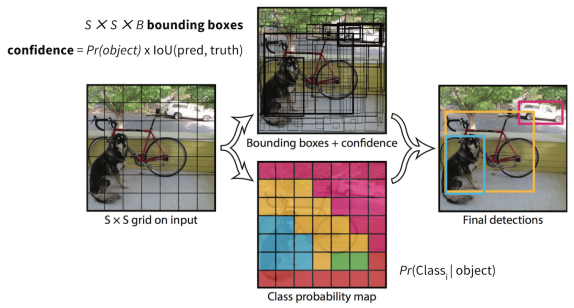
\includegraphics[scale=.6]{32}
		\caption{Ejemplo de uso}
	\end{figure}
	
	La dimensión de salida de YOLO se define como $S*S*(5B+K)$, donde S representa el tamaño de la cuadrícula, B denota el número de cajas de detección por celda, y K es la cantidad de clases de objetos a prever. Este diseño compacto y expresivo es fundamental para la eficiencia y versatilidad del algoritmo.
	

	\subsubsection{Arquitectura}
	La arquitectura de YOLO está organizada en tres etapas fundamentales que abarcan desde la extracción de características hasta la generación de predicciones y el posterior post procesamiento:
		
	\begin{enumerate}
    	\item \textbf{Backbone:} En la primera etapa, YOLO utiliza una red neuronal preentrenada como su espina dorsal o \textit{backbone}. Ejemplos comunes incluyen DarkNet. Esta fase se encarga de extraer características fundamentales de la imagen, aprovechando el conocimiento previo obtenido durante el entrenamiento de la red.

    	\item \textbf{Neck:} La etapa del cuello se caracteriza por capas completamente conectadas que reciben las características extraídas por la espina dorsal. Estas capas se encargan de fusionar y combinar las representaciones de características para capturar información más compleja y contextual. Esta fase actúa como un puente entre la espina dorsal y la capa de salida.

    	\item \textbf{Head:} La última etapa, la cabeza, consiste en la capa de salida que produce las predicciones finales. Aquí se generan las coordenadas de las cajas delimitadoras, las puntuaciones de confianza asociadas a cada detección y las probabilidades de clasificación para las clases de objetos. Además, se aplica el postprocesamiento, que incluye Non-Maximum Suppression (NMS) y el cálculo del Índice de Superposición de Unión (IoU). Estos pasos finales mejoran la precisión y la consistencia de las detecciones, asegurando que se retenga la predicción más confiable y precisa para cada objeto en la imagen.
	\end{enumerate}

	\begin{figure}[ht]
		\centering
		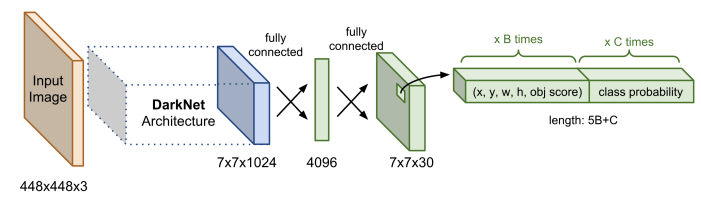
\includegraphics[scale=.6]{33}
		\caption{Ejemplo de arquitectura}
	\end{figure}
	
	\subsubsection{Entrenamiento - Función Pérdida}
	La función de pérdida en la arquitectura YOLO se segmenta en dos componentes fundamentales:
	
	\begin{enumerate}
		\item Pérdida por la predicción del área delimitante $(x, y, h, w)$: $L_loc$
		\item Pérdida por la clasificación del objeto: $L_cls$
	\end{enumerate}
	
	Ambas pérdidas se calculan utilizando el error cuadrático medio (MSE), y cada una de ellas incorpora dos parámetros de escala cruciales: $\lambda_coor$ y $\lambda_noobj$. Estos parámetros influyen en la importancia relativa de cada término de pérdida, permitiendo un ajuste preciso del modelo en función de las metas específicas del entrenamiento.
	\\[0.5cm]
	\textbf{Pérdida en la localización:}
	\vspace{0.5cm}
	\begin{equation*}
		L_{loc} = \lambda_{coord} \sum_{i=0}^{S^2} \sum_{j=0}^{B} 1_{ij}^{obj} [(x_i-\hat{x_i})^2+(y_i-\hat{y_i})^2+(\sqrt{w_i}-\sqrt{\hat{w_i}})^2+(\sqrt{h_i}-\sqrt{\hat{h_i}})^2]
	\end{equation*}
	\vspace{0.1cm}
	\begin{itemize}
		\item \textbf{S}: Cantidad de celdas.
		\item \textbf{B}: Cantidad de áreas de delimitación por celda.
		\item \( \mathbf{1_{ij}^{obj}} \):Indica que el área de delimitación j de la celda i es responsable de la predicción.
	\end{itemize}
	
	\clearpage
	
	\textbf{Pérdida en la clasificación:}
	\vspace{0.5cm}
	\begin{equation*}
		L_{cls} = \lambda_{coord} \sum_{i=0}^{S^2} \sum_{j=0}^{B} (1_{ij}^{obj}+ \lambda_{noobj}(1-1_{ij}^{obj}))(C_{ij}-\hat{C_{ij}})^2+\sum_{i=0}^{S^2} \sum_{c\in{C}} 1_{ij}^{obj}(p_i(c)-\hat{p_i}(c))^2 
	\end{equation*}
	
	\begin{equation*}
		L = L_{loc} + L_{cls}	
	\end{equation*}
	\vspace{0.1cm}
	
	\begin{itemize}
    \item \( \mathbf{1_{i}^{obj}} \): Indica que existe un objeto en la celda \(i\).
    \item \( \mathbf{1_{ij}^{obj}} \): Indica que el área de delimitación \(j\) de la celda \(i\) es responsable de la predicción.
    \item \( \mathbf{C_{ij} }\): Confianza de la celda $(Pr(obj) * IoU(pred, truth))$.
    \item \( \mathbf{\hat{C_{ij}}} \): Confianza de la celda predicha.
    \item \( \mathbf{p_i}(c) \) Probabilidad condicional de una celda \(i\) de contener un objeto de clase \(c\in{C}\).
    \item \( \mathbf{\hat{p_{i}}}(c)\) Probabilidad condicional de una celda \(i\) de contener un objeto de clase \(c\in{C}\) predicha por el modelo
\end{itemize}

	El coeficiente de escala de pérdida $\lambda_{noobj}$ desempeña un papel importante en la prevención de entrenamientos incorrectos, especialmente dado que la mayoría de las celdas en una cuadrícula no contendrán objetos. La determinación del predictor responsable se lleva a cabo mediante el cálculo de la Intersección sobre Unión (IoU). Además, durante el entrenamiento, se emplean cajas de anclaje (anchor boxes) para mejorar y ajustar el rendimiento del predictor.

	\begin{figure}[ht]
		\centering
		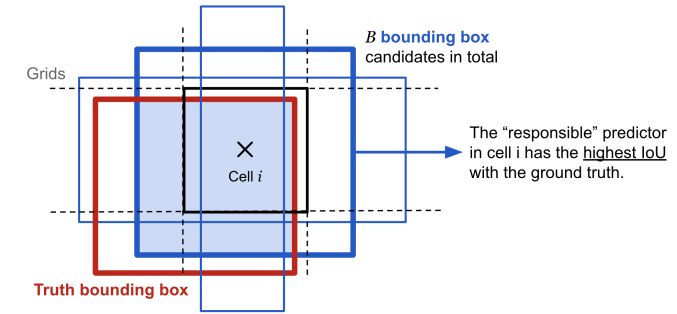
\includegraphics[scale=.6]{34}
		\caption{Representación de la técnica}
	\end{figure}
	
	\subsubsection{Ventajas}
	
	\begin{enumerate}
		\item \textbf{Eficiencia en Tiempo Real:} YOLO es conocido por su eficiencia en tiempo real, ya que realiza la detección de objetos en una sola pasada. Esto lo hace particularmente adecuado para aplicaciones en las que se requiere baja latencia, como en sistemas de vigilancia y conducción autónoma.
    
    	\item \textbf{Detección de Objetos Múltiples:} YOLO puede detectar múltiples objetos en una imagen, incluso aquellos de diferentes tamaños y clases. Su capacidad para manejar la diversidad en la detección es una de sus fortalezas clave.
    
   		\item \textbf{Sim­plicidad y Unificación:} YOLO unifica la clasificación y localización en un solo paso, simplificando el proceso de detección. Su diseño compacto facilita la implementación y el ajuste en diversas aplicaciones.
    
	\end{enumerate}
	
	\subsubsection{Desventajas}
	
	\begin{enumerate}
		\item \textbf{Precisión en Objetos Pequeños:} YOLO puede tener dificultades al detectar objetos pequeños debido a la resolución limitada de las áreas de detección y la pérdida de detalles en objetos diminutos.
    
    	\item \textbf{Manejo de Objetos Superpuestos:} En situaciones donde los objetos están superpuestos, YOLO puede enfrentar desafíos para distinguir y delimitar con precisión cada objeto individual.
    
   	 	\item \textbf{Problema de Clasificación Desbalanceada:} Si hay una gran variabilidad en la cantidad de instancias de diferentes clases en el conjunto de datos, puede haber desafíos asociados con el equilibrio en la clasificación.
    
    	\item \textbf{Entrenamiento Sensible a la Inicialización:} El rendimiento de YOLO puede depender en gran medida de una buena inicialización durante el entrenamiento, y un mal ajuste inicial podría afectar la calidad de las predicciones.	
	
	\end{enumerate}
	
	


	

=======
	Comparado con su predecesor, R-CNN, Faster R-CNN se destaca por su velocidad. Es 250 veces más rápido que R-CNN, y supera significativamente a Fast R-CNN siendo 25 veces más rápido. Estas mejoras en velocidad no solo aceleran el proceso de detección, sino que también abren posibilidades para la implementación de sistemas en tiempo real y aplicaciones de visión por computadora más exigentes.
>>>>>>> Stashed changes

        \begin{flushright}
        \textbf{Material Consultado \cite{cnn}.}
    \end{flushright}
    
\newpage

%----------------------------------------------------------------------------------------
%	IMPLEMENTACIÓN
%----------------------------------------------------------------------------------------
   
\section{Implementación}

    \subsection{Extractor de características}
    Vamos a emplear una red pre-entrenada, específicamente la 'VGG16', como extractor de características para una imagen de entrada con dimensiones de 400x240 píxeles y 3 canales, previamente normalizada. En este caso, hemos truncado la red hasta la capa 'block4-conv3', generando así un mapa de características de 30x50 con 512 características. Con esta configuración, al aplicar la ventana deslizante, obtenemos \textbf{30 filas y 50 columnas}. Donde cada ventana corresponde a una dimensión en la imagen original de \textbf{8x8 píxeles}.

    A continuación se representará gráficamente al modelo truncado para nuestra aplicación:

    \vspace{0.4cm}
    
    \begin{figure}[ht]
	    \centering
		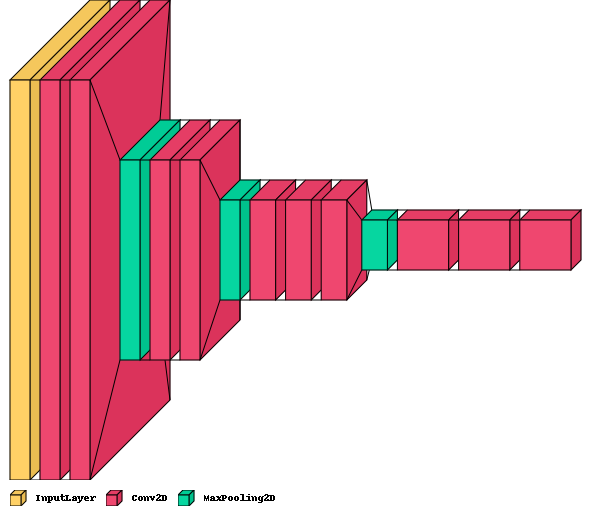
\includegraphics[scale=0.4]{img/VGG16.png}
		\caption{Arquitectura del extractor de características}
	\end{figure}

    \subsection{Dataset y Modelo ROI ``Region Of Interest''}
    Este modelo se compone exclusivamente de una red totalmente conectada que emplea la salida del extractor de características en conjunto con una ventana deslizante. Por lo tanto recibe mapas de características de dimensiones 1x1x512 y genera predicciones binarias para determinar la presencia o ausencia de una señal de tránsito en cada ventana.

    A continuación se representará gráficamente al modelo:
    
    \vspace{0.5cm}

    \begin{figure}[ht]
        \centering
        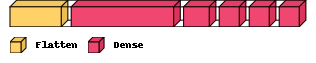
\includegraphics[scale=0.85]{ROI Model.png}
        \caption{Arquitectura del modelo ROI}
    \end{figure}

    \vspace{0.2cm}

    Para el entrenamiento de esta red, se procedió a generar un dataset que contiene mapas de características de las señales de tránsito y de las que no son señales, cada uno con su respectiva etiqueta.
    Se sabe que la salida del extractor de características genera un mapa con una dimensión determinada, donde cada ``píxel'' o 1x1x512 representa en la imágen original una dimensión de 16x16 píxeles y 3 canales.

    \pagebreak
    
    \begin{figure}[ht]
        \centering
        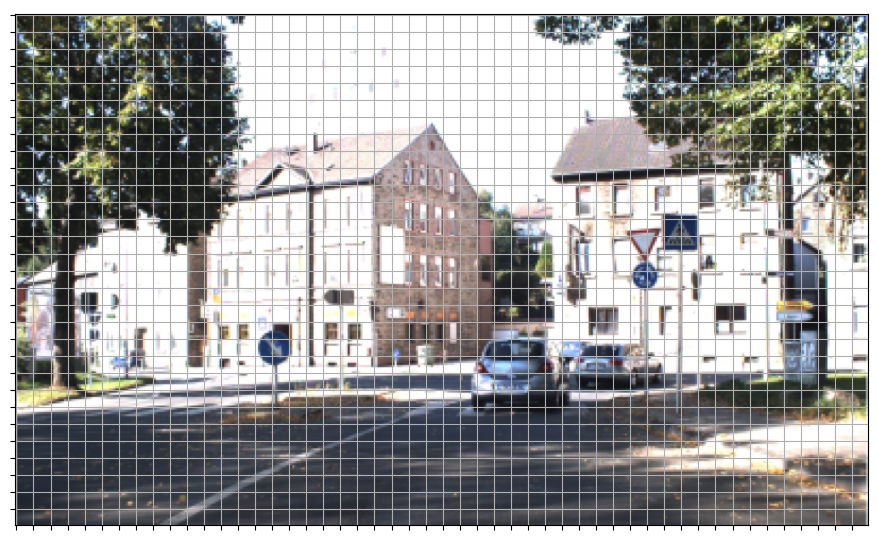
\includegraphics[scale=0.40]{Grid.png}
        \caption{Grilla Generada por el extractor de características}
    \end{figure}

    También se conoce la ubicación de cada señal de tránsito, la cual es obtenida en la documentación del dataset.

    \begin{figure}[ht]
        \centering
        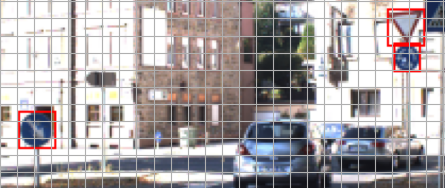
\includegraphics[scale=.8]{img/Grid_label.png}
        \caption{Grilla y Ubicación de las Señales de Tránsito}
    \end{figure}

    Por lo que habrá que definir una métrica para determinar si en cada cuadrante de la grilla, este pertenece o no a una señal de tránsito, para eso se consideró la métrica de la Intersección sobre la Unión y la de solamente el porcentaje de intersección:
    
    \begin{figure}[ht]
        \centering
        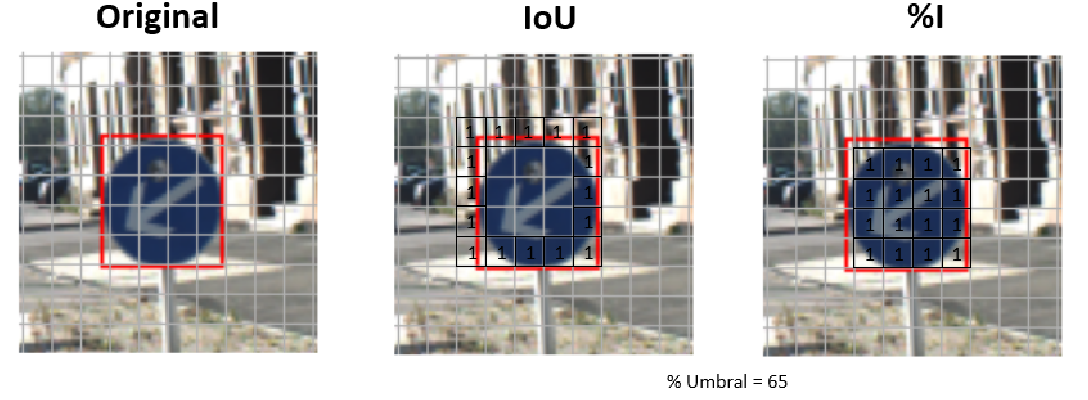
\includegraphics[scale=0.4]{I.png}
        \caption{IoU vs. I}
    \end{figure}

    Como se aprecia, la métrica del porcentaje de intersección en este caso es mucho mejor, ya que en el caso de la intersección sobre la unión, se eliminarán datos de suma importancia como es el interior de la señal de tránsito.

    Para la generación de los mapas de características de las señales de tránsito, simplemente debemos extraer el mapa de característica en cada columna y fila donde el binarizado de la métrica sea 1. En cambio para los mapas de características de aquellas partes donde no se encuentra una señal de tránsito, se utilizó un generador aleatorio de números enteros para colocarlos en la grilla con el cuidado de que este generador no nos de un par fila-columna tal que sea una señal de tránsito, este generador aleatorio fue puesto con una distribución normal con media la mitad de la grilla y varianza 4; Esto nos permite obtener más información del centro de la imagen y en zonas donde es más probable encontrar una señal de tránsito.

    La estructura del dataset es la siguiente:
    
    \begin{figure}[ht]
        \centering
        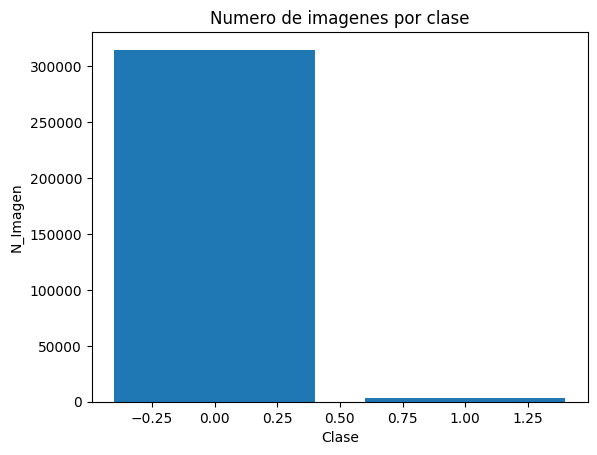
\includegraphics[scale=0.5]{Clases_ROI.png}
        \caption{Estructura del Dataset ROI}
    \end{figure}


    \subsection{Dataset y Modelo del Clasificador}
    Se empleó el conjunto de datos GTSRB, el cual proporciona información tanto para el entrenamiento como para la prueba, incluyendo etiquetas asociadas.

    El conjunto de datos de entrenamiento consta de 39,209 imágenes de tamaño variable, representando señales de tránsito capturadas desde diversas cámaras, bajo condiciones de iluminación y ángulos diversos. 
    Este conjunto abarca 43 clases distintas para su clasificación, pero se agregó una clase adicional para eliminar falsos positivos, esta clase es la denominada ``Nada'' y la obtuvimos mediante el dataset ``JCNN'' generando recortes de imágenes que no fueran señales de tránsito conociendo las regiones de la imágen que sí contienen señales de tránsito, tal información se recopiló en la documentación de los datasets, por lo tanto, todo este conjunto de datos que se utilizó para entrenar el clasificador posee la siguiente estructura:
    
    \begin{figure}[ht]
	    \centering
		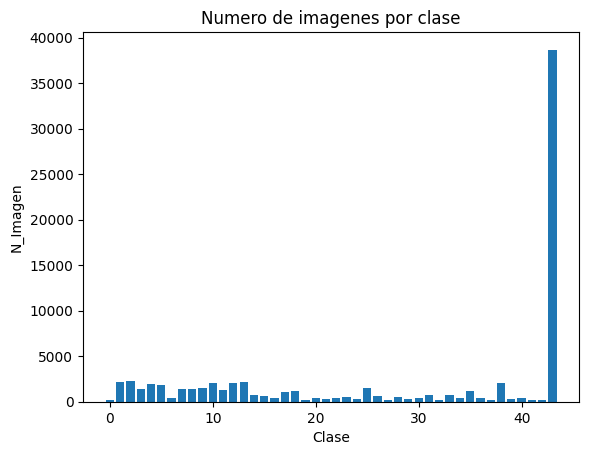
\includegraphics[scale=.55]{img/Clases.png}
		\caption{Estructura del Dataset}
	\end{figure}
 
    Es evidente que este conjunto de datos presenta un desequilibrio, lo que significa que no hay una distribución equitativa de datos para cada clase. Esta asimetría se ha diseñado con un propósito específico relacionado con la probabilidad de ocurrencia de cada clase. En consecuencia, la clase con menos datos tendrá una probabilidad menor de aparecer. Se puede equilibrar este conjunto de datos de forma artificial en el entrenamiento, ajustando las ponderaciones por cada clase.

    Previo al entrenamiento del modelo clasificador, cada imagen requiere de un pre-procesamiento; Se debe ajustar su dimensión a 32x32 píxeles y normalizarla. La normalización implica modificar el rango de cada canal de color de 0 a 255 a un nuevo rango de 0 a 1, garantizando así una representación estandarizada de los datos.

    En cuanto al modelo del clasificador, definimos la siguiente arquitectura de una red convolucional:

    \begin{figure}[ht]
	    \centering
		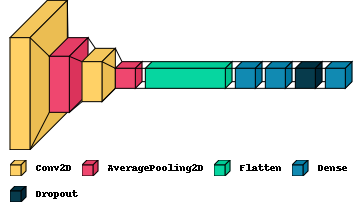
\includegraphics[scale=0.6]{img/GTSRB.png}
		\caption{Arquitectura del clasificador}
	\end{figure}
 
    Al entrenar el modelo y establecer una tasa de aprendizaje inicial lo suficientemente baja, se logra:

    \begin{figure}[ht]
	    \centering
		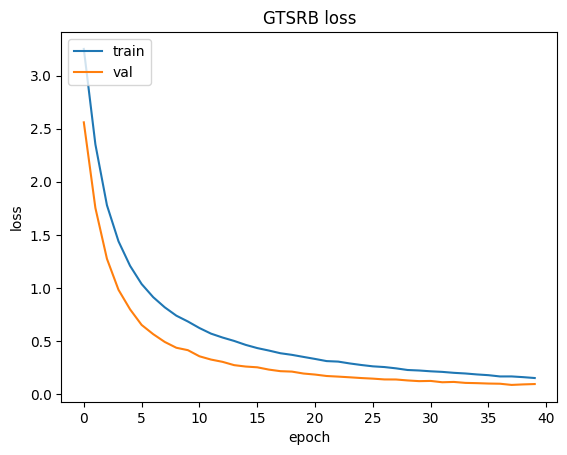
\includegraphics[scale=0.45]{img/GTSRB_Loss.png}
		\caption{Pérdida del modelo}
	\end{figure}
    
    A continuación, se incluirán algunas predicciones generadas por el modelo propuesto utilizando el conjunto de datos de prueba, con el objetivo de verificar su capacidad de generalización adecuada:
    
    \begin{figure}[ht]
	    \centering
		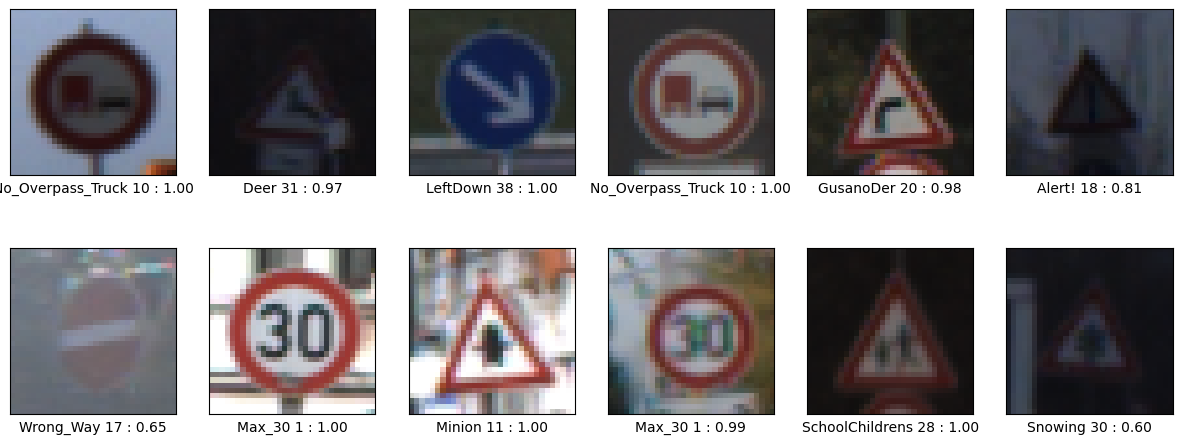
\includegraphics[scale=0.3]{img/GTSRB_Pred.png}
		\caption{Prueba del modelo}
	\end{figure}

    En la imagen previa, se presenta la clase asignada a cada imagen, acompañada del correspondiente porcentaje de confianza proporcionado por el modelo en su respectiva predicción.


%----------------------------------------------------------------------------------------
%	RESULTADOS
%----------------------------------------------------------------------------------------
\newpage
\section{Resultados}
    \subsection{Extractor de características}
    Como antes se ha mencionado se genera un mapa de 30x50 con 512 características, de cada una de las imágenes del dataset GTSRB, gracias a la red neuronal convolucional VGG-16. Algo a destacar es que estas características de las imágenes son a nivel teórico para nosotros los bordes, tamaños, texturas, patrones entre otros. Pero a nivel máquina, lo que puede visualizarse como características son figuras sin sentido.

    Por ejemplo tomemos una imágen del dataset GTSRB y veamos un mapa de característica.


    \begin{figure}[ht]
			\centering
			\begin{subfigure}[t]{.47\textwidth}
				\centering
				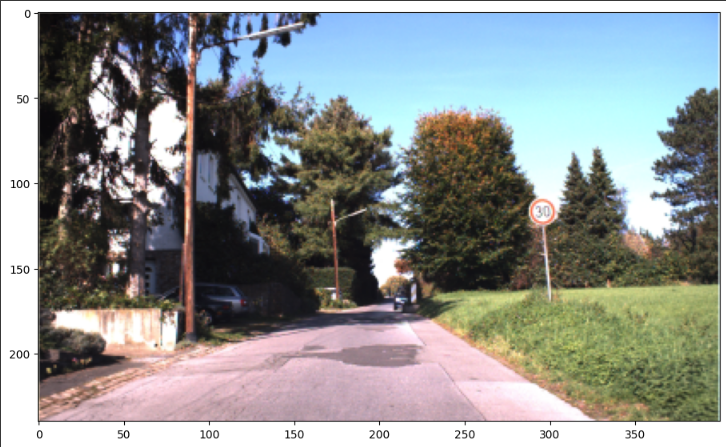
\includegraphics[scale=.35]{example_GTSRB.png}
                \caption{Imagen extraída del dataset}
			\end{subfigure}
			\begin{subfigure}[t]{.47\textwidth}
				\centering
				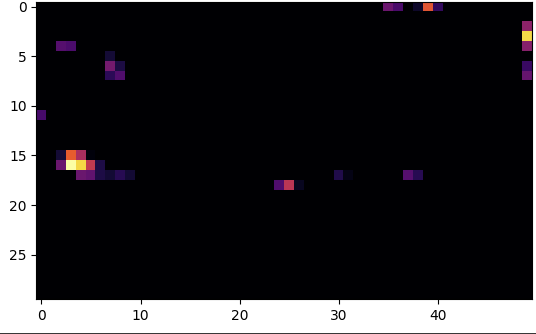
\includegraphics[scale=.47]{map.png}
                \caption{Un mapa de características de la imagen}
			\end{subfigure}
			\caption{Extracción de un mapa de característica}
	\end{figure}	


    \subsection{Region Of Intereset}
    Como ya se ha mencionado, la capa ROI Pooling recibe mapas de características de dimensiones 1x1x512 generados por la red VGG-16 para cada imagen en el conjunto de datos GTSRB. Estos mapas representan abstracciones a nivel de bordes, tamaños, texturas y patrones. La capa ROI Pooling procesa selectivamente estas características y produce predicciones binarias que indican la presencia o ausencia de señales de tránsito en regiones específicas de la imagen.
    
    Por ejemplo, si tomamos una imagen del dataset GTSRB con su respectiva matriz ROI resulta lo siguiente:

    \begin{figure}[ht]
			\centering
			\begin{subfigure}[t]{.47\textwidth}
				\centering
				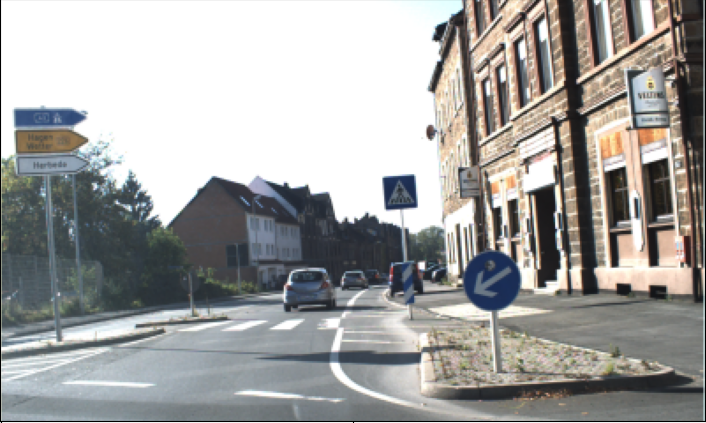
\includegraphics[scale=.35]{Imagen sin procesar para ROI.png}
                \caption{Imagen original}
			\end{subfigure}
			\begin{subfigure}[t]{.47\textwidth}
				\centering
				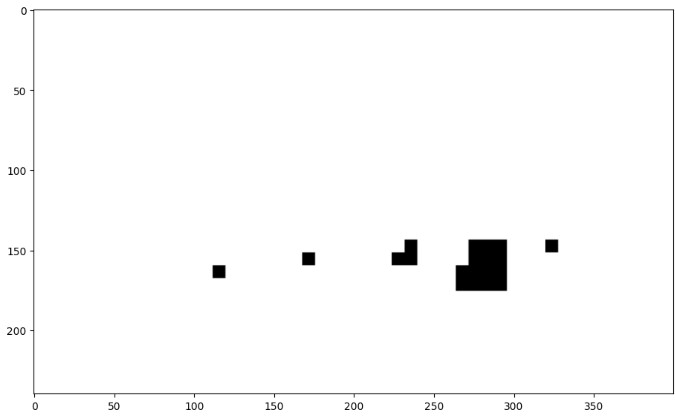
\includegraphics[scale=.35]{Matriz unos y ceros.jpg}
                \caption{Mapa de unos y ceros de la imagen}
			\end{subfigure}
	\end{figure}	
    Lo que se puede observar entonces es una imagen blanca con pequeñas "manchas negras", que representan aquellas regiones de la imagen en donde puede haber características de interés (en este caso, posibles señales de tránsito).

    \subsubsection{Métricas}

    A continuación se verán reflejadas algunas métricas que se utilizaron para evaluar el modelo. Cabe recalcar que como el dataset se encuentra desbalanceado (muchos ceros y pocos unos), las métricas de accuracy y matriz de confusión suelen arrojar resultados bastante favorables. Es por ello que por lo general se presta mayor atención a la métrica referente a la pérdida del modelo.
    \pagebreak

    A partir de lo expuesto a continuación por los gráficos de pérdida y accuracy del modelo, puede observarse que el modelo no está sobre entrenado (overfitting) ya que las curvas de entrenamiento y validación convergen a valores muy similares luego del entrenamiento.

    \vspace{0.2cm}

    \begin{figure}[ht]
			\centering
			\begin{subfigure}[t]{.47\textwidth}
        	    \centering
        		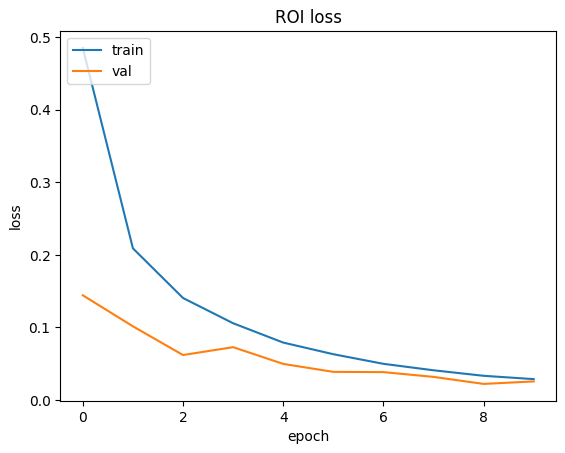
\includegraphics[scale=0.38]{Loss.png}
        		\caption{Pérdida del modelo}
			\end{subfigure}
			\begin{subfigure}[t]{.47\textwidth}
        	    \centering
        		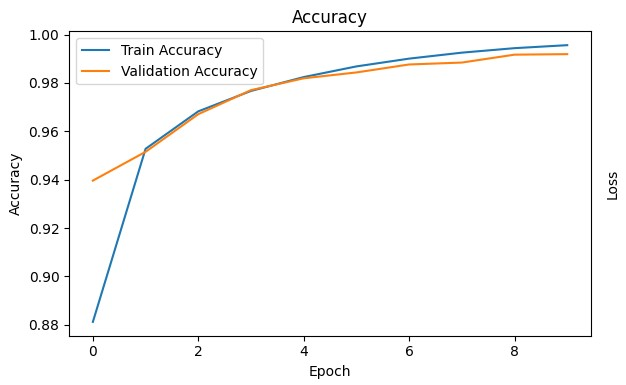
\includegraphics[scale=0.45]{Grafico accuracy ROI.jpg}
        		\caption{Accuracy del modelo}
			\end{subfigure}
	\end{figure}	

    \vspace{0.2cm}
 
    Para la métrica \textbf{matriz de confusión} se ha separado del dataset de entrenamiento un cierto porcentaje de datos para la validación del modelo.

    Podemos observar que en el eje \texttt{X} nos encontramos con las \textbf{Etiquetas Predichas} por el modelo y en el eje \texttt{Y} con las \textbf{Etiquetas Reales}.

    La \textbf{matriz de confusión} nos dice que el modelo predice correctamente que se han detectado 15655 \textbf{0's} y 147 \textbf{1's}, sin embargo también hay  7 \textbf{falsos negativos} y 94 \textbf{falsos positivos}.

    \vspace{0.4cm}
    
    \begin{figure}[ht]
	    \centering
		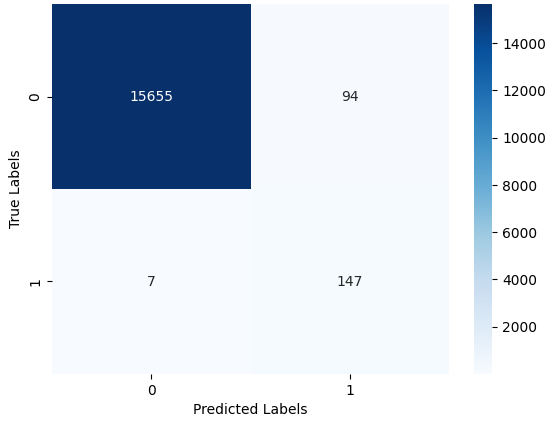
\includegraphics[scale=0.5]{Confusion_Matrix.png}
		\caption{Matriz de Confusión}
	\end{figure}

    
    \subsection{Modelo de Detección y Clasificación de Señales}
    El modelo de detección de señales de tránsito es un sistema completo hecho para procesar imágenes originales y realizar la identificación y clasificación de señales de tránsito presentes en la escena.

    Además, la entrada del modelo consiste en la imagen original capturada, que puede contener diversas señales de tránsito en diferentes contextos y condiciones de iluminación.

    Por otro lado, la salida final del modelo incluye la imagen original con las señales de tránsito recuadradas y etiquetadas, mostrando visualmente cómo resultan la detección y clasificación de las señales presentes en la escena.

    \pagebreak

    Por ejemplo, así es como el modelo procesa una de las imágenes del dataset:

    \begin{figure}[ht]
			\centering
			\begin{subfigure}[t]{.47\textwidth}
				\centering
				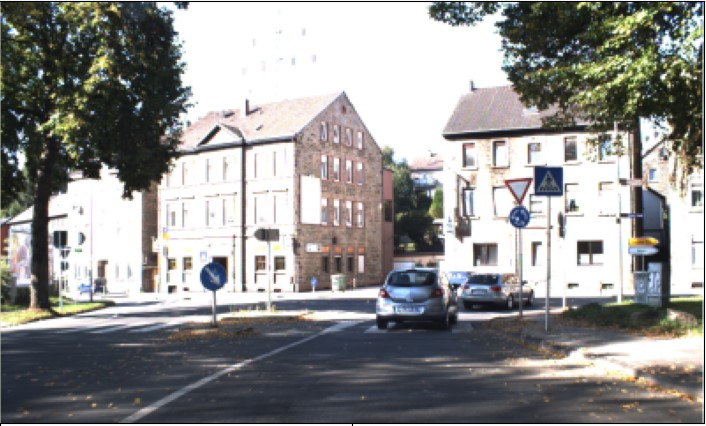
\includegraphics[scale=.39]{Imagen sin procesar.jpg}
                \caption{Imagen sin procesar}
			\end{subfigure}
			\begin{subfigure}[t]{.47\textwidth}
				\centering
				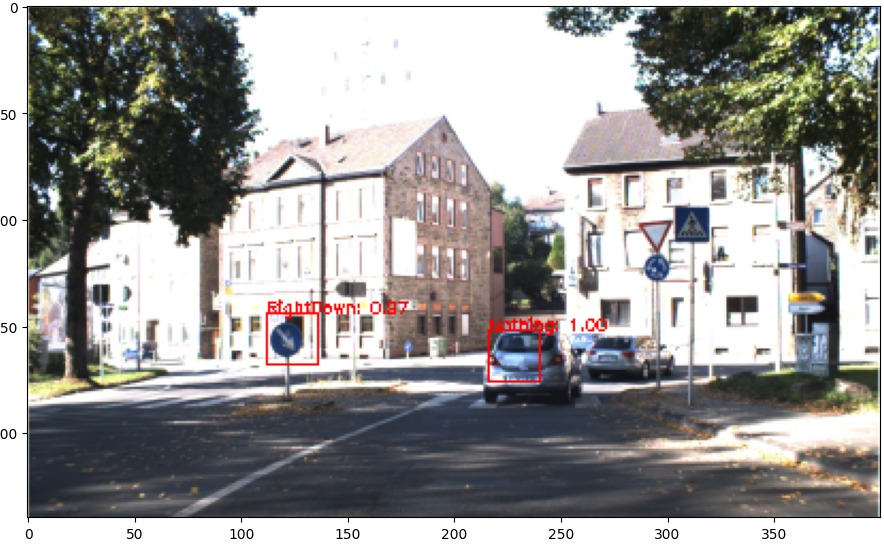
\includegraphics[scale=.23]{Imagen procesada.jpeg}
                \caption{Imagen procesada}
			\end{subfigure}
			\caption{Procesamiento de una imagen}
	\end{figure}	

    \subsection{Arquitectura del modelo total}

    \begin{figure}[ht]
	    \centering
		\includegraphics[scale=0.53]{final.png}
		\caption{Implementación del modelo final}
	\end{figure}

 \vspace{0.5cm}

 \subsection{Plataforma de implementación}
 La implementación del trabajo \textbf{Redes Neuronales: Aplicada a la detección de señales de tránsito} se llevó a cabo en la plataforma Google Colab. El link se encuentra en \cite{colab}

%----------------------------------------------------------------------------------------
%	CONCLUSIÓN
%----------------------------------------------------------------------------------------
\newpage
\section{Conclusión}
En este proyecto de detección de señales de tránsito, hemos implementado una arquitectura que utiliza la red neuronal convolucional VGG-16 junto con la capa ROI Pooling. A través de este enfoque, hemos logrado identificar regiones de interés en las imágenes, interpretando estas áreas como posibles señales de tránsito.

La capa ROI Pooling, ha sido de utilidad en el procesamiento selectivo de estas regiones, generando predicciones binarias sobre la presencia de señales. La inclusión de un componente de clasificación ha proporcionado etiquetas asociadas con las señales detectadas.

Los resultados obtenidos indican que la arquitectura es capaz de abordar la tarea de detección y clasificación de señales de tránsito. Sin embargo, y aunque los resultados obtenidos son alentadores, reconocemos la necesidad de mejorar la robustez de nuestro modelo ROI, especialmente en situaciones donde las señales son demasiado cercanas entre sí. Un modelo más sofisticado podría abordar estos desafíos, mejorando la capacidad de discernir señales adyacentes y optimizando la precisión general del sistema.

Adicionalmente, consideramos que el rendimiento de nuestro modelo podría beneficiarse significativamente de entornos de ejecución más potentes. Con recursos computacionales adicionales, podríamos procesar imágenes de mayor resolución, lo que permitiría la detección de señales a mayores distancias.